% Options for packages loaded elsewhere
\PassOptionsToPackage{unicode}{hyperref}
\PassOptionsToPackage{hyphens}{url}
%
\documentclass[
  man,floatsintext]{apa6}
\usepackage{amsmath,amssymb}
\usepackage{iftex}
\ifPDFTeX
  \usepackage[T1]{fontenc}
  \usepackage[utf8]{inputenc}
  \usepackage{textcomp} % provide euro and other symbols
\else % if luatex or xetex
  \usepackage{unicode-math} % this also loads fontspec
  \defaultfontfeatures{Scale=MatchLowercase}
  \defaultfontfeatures[\rmfamily]{Ligatures=TeX,Scale=1}
\fi
\usepackage{lmodern}
\ifPDFTeX\else
  % xetex/luatex font selection
\fi
% Use upquote if available, for straight quotes in verbatim environments
\IfFileExists{upquote.sty}{\usepackage{upquote}}{}
\IfFileExists{microtype.sty}{% use microtype if available
  \usepackage[]{microtype}
  \UseMicrotypeSet[protrusion]{basicmath} % disable protrusion for tt fonts
}{}
\makeatletter
\@ifundefined{KOMAClassName}{% if non-KOMA class
  \IfFileExists{parskip.sty}{%
    \usepackage{parskip}
  }{% else
    \setlength{\parindent}{0pt}
    \setlength{\parskip}{6pt plus 2pt minus 1pt}}
}{% if KOMA class
  \KOMAoptions{parskip=half}}
\makeatother
\usepackage{xcolor}
\usepackage{graphicx}
\makeatletter
\def\maxwidth{\ifdim\Gin@nat@width>\linewidth\linewidth\else\Gin@nat@width\fi}
\def\maxheight{\ifdim\Gin@nat@height>\textheight\textheight\else\Gin@nat@height\fi}
\makeatother
% Scale images if necessary, so that they will not overflow the page
% margins by default, and it is still possible to overwrite the defaults
% using explicit options in \includegraphics[width, height, ...]{}
\setkeys{Gin}{width=\maxwidth,height=\maxheight,keepaspectratio}
% Set default figure placement to htbp
\makeatletter
\def\fps@figure{htbp}
\makeatother
\setlength{\emergencystretch}{3em} % prevent overfull lines
\providecommand{\tightlist}{%
  \setlength{\itemsep}{0pt}\setlength{\parskip}{0pt}}
\setcounter{secnumdepth}{-\maxdimen} % remove section numbering
% Make \paragraph and \subparagraph free-standing
\ifx\paragraph\undefined\else
  \let\oldparagraph\paragraph
  \renewcommand{\paragraph}[1]{\oldparagraph{#1}\mbox{}}
\fi
\ifx\subparagraph\undefined\else
  \let\oldsubparagraph\subparagraph
  \renewcommand{\subparagraph}[1]{\oldsubparagraph{#1}\mbox{}}
\fi
\newlength{\cslhangindent}
\setlength{\cslhangindent}{1.5em}
\newlength{\csllabelwidth}
\setlength{\csllabelwidth}{3em}
\newlength{\cslentryspacingunit} % times entry-spacing
\setlength{\cslentryspacingunit}{\parskip}
\newenvironment{CSLReferences}[2] % #1 hanging-ident, #2 entry spacing
 {% don't indent paragraphs
  \setlength{\parindent}{0pt}
  % turn on hanging indent if param 1 is 1
  \ifodd #1
  \let\oldpar\par
  \def\par{\hangindent=\cslhangindent\oldpar}
  \fi
  % set entry spacing
  \setlength{\parskip}{#2\cslentryspacingunit}
 }%
 {}
\usepackage{calc}
\newcommand{\CSLBlock}[1]{#1\hfill\break}
\newcommand{\CSLLeftMargin}[1]{\parbox[t]{\csllabelwidth}{#1}}
\newcommand{\CSLRightInline}[1]{\parbox[t]{\linewidth - \csllabelwidth}{#1}\break}
\newcommand{\CSLIndent}[1]{\hspace{\cslhangindent}#1}
\ifLuaTeX
\usepackage[bidi=basic]{babel}
\else
\usepackage[bidi=default]{babel}
\fi
\babelprovide[main,import]{english}
% get rid of language-specific shorthands (see #6817):
\let\LanguageShortHands\languageshorthands
\def\languageshorthands#1{}
% Manuscript styling
\usepackage{upgreek}
\captionsetup{font=singlespacing,justification=justified}

% Table formatting
\usepackage{longtable}
\usepackage{lscape}
% \usepackage[counterclockwise]{rotating}   % Landscape page setup for large tables
\usepackage{multirow}		% Table styling
\usepackage{tabularx}		% Control Column width
\usepackage[flushleft]{threeparttable}	% Allows for three part tables with a specified notes section
\usepackage{threeparttablex}            % Lets threeparttable work with longtable

% Create new environments so endfloat can handle them
% \newenvironment{ltable}
%   {\begin{landscape}\centering\begin{threeparttable}}
%   {\end{threeparttable}\end{landscape}}
\newenvironment{lltable}{\begin{landscape}\centering\begin{ThreePartTable}}{\end{ThreePartTable}\end{landscape}}

% Enables adjusting longtable caption width to table width
% Solution found at http://golatex.de/longtable-mit-caption-so-breit-wie-die-tabelle-t15767.html
\makeatletter
\newcommand\LastLTentrywidth{1em}
\newlength\longtablewidth
\setlength{\longtablewidth}{1in}
\newcommand{\getlongtablewidth}{\begingroup \ifcsname LT@\roman{LT@tables}\endcsname \global\longtablewidth=0pt \renewcommand{\LT@entry}[2]{\global\advance\longtablewidth by ##2\relax\gdef\LastLTentrywidth{##2}}\@nameuse{LT@\roman{LT@tables}} \fi \endgroup}

% \setlength{\parindent}{0.5in}
% \setlength{\parskip}{0pt plus 0pt minus 0pt}

% Overwrite redefinition of paragraph and subparagraph by the default LaTeX template
% See https://github.com/crsh/papaja/issues/292
\makeatletter
\renewcommand{\paragraph}{\@startsection{paragraph}{4}{\parindent}%
  {0\baselineskip \@plus 0.2ex \@minus 0.2ex}%
  {-1em}%
  {\normalfont\normalsize\bfseries\itshape\typesectitle}}

\renewcommand{\subparagraph}[1]{\@startsection{subparagraph}{5}{1em}%
  {0\baselineskip \@plus 0.2ex \@minus 0.2ex}%
  {-\z@\relax}%
  {\normalfont\normalsize\itshape\hspace{\parindent}{#1}\textit{\addperi}}{\relax}}
\makeatother

% \usepackage{etoolbox}
\makeatletter
\patchcmd{\HyOrg@maketitle}
  {\section{\normalfont\normalsize\abstractname}}
  {\section*{\normalfont\normalsize\abstractname}}
  {}{\typeout{Failed to patch abstract.}}
\patchcmd{\HyOrg@maketitle}
  {\section{\protect\normalfont{\@title}}}
  {\section*{\protect\normalfont{\@title}}}
  {}{\typeout{Failed to patch title.}}
\makeatother

\usepackage{xpatch}
\makeatletter
\xapptocmd\appendix
  {\xapptocmd\section
    {\addcontentsline{toc}{section}{\appendixname\ifoneappendix\else~\theappendix\fi\\: #1}}
    {}{\InnerPatchFailed}%
  }
{}{\PatchFailed}
\keywords{listener design, knowledge inference, social class}
\usepackage{lineno}

\linenumbers
\usepackage{csquotes}
\ifLuaTeX
  \usepackage{selnolig}  % disable illegal ligatures
\fi
\IfFileExists{bookmark.sty}{\usepackage{bookmark}}{\usepackage{hyperref}}
\IfFileExists{xurl.sty}{\usepackage{xurl}}{} % add URL line breaks if available
\urlstyle{same}
\hypersetup{
  pdftitle={Knowledge Inference and Social Class Common Ground},
  pdfauthor={Sooyoun Zong1},
  pdflang={en-EN},
  pdfkeywords={listener design, knowledge inference, social class},
  hidelinks,
  pdfcreator={LaTeX via pandoc}}

\title{Knowledge Inference and Social Class Common Ground}
\author{Sooyoun Zong\textsuperscript{1}}
\date{}


\shorttitle{Social Class and Conversational Cues}

\authornote{

Please email \href{mailto:krstnnna@uchicago.edu}{\nolinkurl{krstnnna@uchicago.edu}} for questions about this important research.

}

\affiliation{\vspace{0.5cm}\textsuperscript{1} University of Chicago}

\abstract{%
This study explores the nuanced way in which social class is inferred from conversational cues. Grounded in the disciplines of psychology and sociolinguistics, I examine how speakers' adjusted language allows third-party evaluators to draw inferences about the listener's social class. Through an experimental design involving vignettes that vary in the level of explanation provided, the research seeks to uncover the cognitive processes underlying the perception of social class from brief speech samples and the potential impact of these perceptions on judgments about a person's competence and social identity. This investigation into the subtleties of language and social signaling offers insights into the reproduction of stratification through everyday interactions.
}



\begin{document}
\maketitle

\hypertarget{knowledge-inference-and-social-class-common-ground}{%
\section{Knowledge Inference and Social Class Common Ground}\label{knowledge-inference-and-social-class-common-ground}}

In the realm of social interaction, our linguistic, behavioral, and cultural markers play a pivotal role in conveying our social identity, with research highlighting the ability of humans to discern others' social status through verbal and nonverbal cues. Sebastian and Bouchard Ryan (2018) have shown that language cues like accent, tone, and linguistic variations are key in revealing a speaker's ethnicity, social class, and age, while Bjornsdottir and Rule (2017) found that facial cues alone allow perceivers to accurately categorize individuals as rich or poor, often employing stereotype-related impressions in their judgments. Kraus, Torrez, Park, and Ghayebi (2019) further demonstrated that social class signals are effectively communicated through brief speech samples, emphasizing pronunciation as a significant indicator. This body of work suggests that social class can be inferred not only from one's speech or appearance but also from how others interact with and address the individual, indicating a broader, more nuanced understanding of social class perception.

The concept of listener design in sociolinguistics, which involves speakers tailoring their speech patterns and utterances to their audience's perceived knowledge and background, further enriches the discussion on communication and social identity. This adaptability in communication aims to establish social rapport and ensure clarity across diverse social contexts, guided by the speaker's and listener's social identities and the interpersonal dynamics at play. The notion of class-specific common knowledge underscores that individuals from different social classes possess distinct information and experiences, influencing the social circles they engage with and the societal norms they follow. Therefore, effective communication in diverse social settings necessitates an awareness of each other's social class background, highlighting the role of listener design in revealing and navigating social class perceptions.

\hypertarget{the-present-analysis}{%
\section{The Present Analysis}\label{the-present-analysis}}

Built upon the premise of the listener design---that the speaker correctly assumes and accommodates language to the listener, this study aims to demonstrate that the speaker's words may inform the third party of the listener's knowledge and social class. In specific objective of this analysis is to capture people's sense of class-specific knowledge. Identifying the listener's social class from the inferred knowledge will entail their recognition of the common ground that different social class groups possess.

The experiment will be constructed on the following logic: (1) The speaker's basic explanation of a topic (that a particular social class group typically knows) implies the listener's lack of knowledge. (2) The listener's lack of certain knowledge indicates his or her distance from that social class group.

\hypertarget{methods}{%
\section{Methods}\label{methods}}

\hypertarget{participants}{%
\subsection{Participants}\label{participants}}

100 participants from various socioeconomic backgrounds taok part in this study. The participants were recruited online and compensated through Prolific, a widely used recruitment platform for social research.

\hypertarget{procedure}{%
\subsection{Procedure}\label{procedure}}

I created vignettes of two individuals having a conversation, where a particular topic comes up, and one person clarifies. The topics are expected to differ significantly regarding knowledge or experience based on social class. Participants (``Evaluators'') read one of the two (higher-class and lower-class) vignettes of conversation and were asked to report their perception of the listener's social class as well as their knowledge of the topic being discussed.

\hypertarget{measures}{%
\subsection{Measures}\label{measures}}

\hypertarget{manipulation-check}{%
\subsubsection{Manipulation check}\label{manipulation-check}}

After reading each vignette, participants indicated their knowledge of the topic on a 5-point Likert scale (1 = no knowledge, 5 = thorough knowledge).

\hypertarget{listeners-social-class-rating}{%
\subsubsection{Listener's social class rating}\label{listeners-social-class-rating}}

Participants were asked to identify the listener's social class using the MacArthur Scale of Subjective Socioeconomic Status (Adler et al., 2000), which shows ten rungs representing U.S. society. Participants indicated the position in which the listener would be placed.

\hypertarget{demographic-backgrounds}{%
\subsubsection{Demographic backgrounds}\label{demographic-backgrounds}}

Social identities of all contributors influence the dynamics of speech-based class perception (Stephens et al., 2019). Participants reported their subjective social class at the end of survey as well.

\hypertarget{analysis}{%
\section{Analysis}\label{analysis}}

\hypertarget{overall-descriptive-statistics}{%
\subsection{Overall Descriptive Statistics}\label{overall-descriptive-statistics}}

\begin{table}[!h]
\centering
\caption{\label{tab:descriptive-statistics}Descriptive Statistics of Evaluators' Average Social class, Knowledge, and Rating}
\centering
\begin{tabular}[t]{ccccccc}
\toprule
Vignette & Class & SD & Knowledge & SD & Listener Class Rating & SD\\
\midrule
Higher-Class & 4.73 & 1.48 & 3.17 & 0.70 & 6.57 & 1.91\\
Lower-Class & 5.03 & 1.73 & 3.08 & 0.81 & 4.83 & 1.72\\
\bottomrule
\end{tabular}
\end{table}

To examine the relationship between an evaluator's social class and their knowledge of the specific conversation topic, I implemented a two-fold analysis. The first part of the analysis utilized correlation analysis within each vignette\footnote{The analyses and visualizations were conducted using R's ggplot() function.} and the second part employed independent samples t-test between two groups of evaluators categorized by social class\footnote{The analysis was conducted using R's t.test() function.}. This dual approach aimed to verify two hypotheses: firstly, whether a higher social class correlates with increased knowledge about the topic typically associated with the upper class, and secondly, if an evaluator's social class (higher or lower) could predict their knowledge level on the topic related to their respective social classes.

Next, the difference in listener's social class rating was also assessed by independent samples t-test between two vignettes\footnote{The analysis was conducted using R's t.test() function.}. This revealed whether evaluators were able to accurately infer the social class of listener from the conversation.

Tables are used to present a more detailed quantitative analysis. These include descriptive statistics and summaries of t-test results, which provide a comprehensive overview of the statistical relationships. Complementing the statistical data, I employed several types of plots to visually represent the findings\footnote{The analyses and visualizations were conducted using R's ggplot() function.}. Scatter plots with fitted lines are used to illustrate the relationship between social class and knowledge on higher-class topics, offering a visual representation of any positive or negative correlations. Bar plots with error bars are generated, with each bar representing the mean level of a group, allowing for a clear comparison of mean levels between two groups.

\hypertarget{evaluator-knowledge-correlation-with-social-class}{%
\subsection{Evaluator Knowledge: Correlation with Social Class}\label{evaluator-knowledge-correlation-with-social-class}}

\begin{figure}
\centering
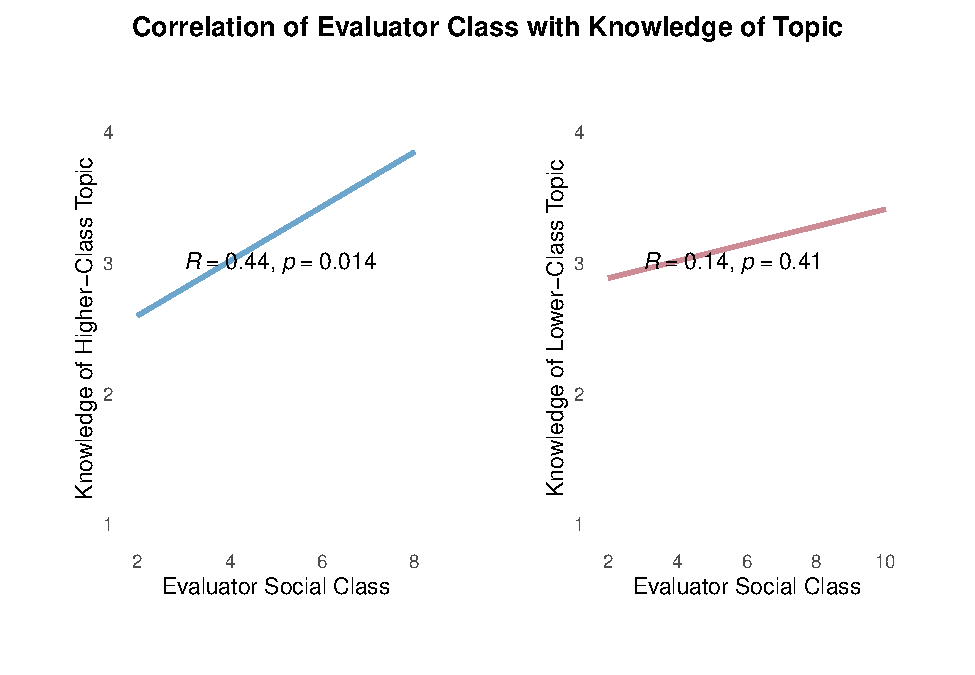
\includegraphics{sooyoun-pilot_files/figure-latex/correlation-analysis-1.pdf}
\caption{\label{fig:correlation-analysis}Correlation Between Evaluator Class and Knowledge}
\end{figure}

The analysis revealed a significant correlation for the higher-class vignette (r = .44, p = .014), indicating a strong relationship between social class and knowledge of topics typically associated with higher-class contexts. No significant correlation was found for the lower-class vignette (r = .14, p = .041).

\hypertarget{evaluator-knowledge-comparison-by-social-class}{%
\subsection{Evaluator Knowledge: Comparison by Social Class}\label{evaluator-knowledge-comparison-by-social-class}}

\begin{table}[!h]
\centering
\caption{\label{tab:group-statistics}Summary Statistics of Evaluator Knowledge of Higher-Class Topic}
\centering
\begin{tabular}[t]{ccccc}
\toprule
Social Class & Mean & SD & sem & N\\
\midrule
Higher-Class & 3.43 & 0.53 & 0.20 & 7\\
Lower-Class & 3.09 & 0.73 & 0.15 & 23\\
\bottomrule
\end{tabular}
\end{table}

\begin{table}[!h]
\centering
\caption{\label{tab:group-statistics}Summary Statistics of Evaluator Knowledge of Lower-Class Topic}
\centering
\begin{tabular}[t]{ccccc}
\toprule
Social Class & Mean & SD & sem & N\\
\midrule
Higher-Class & 3.36 & 0.67 & 0.20 & 11\\
Lower-Class & 2.96 & 0.84 & 0.17 & 25\\
\bottomrule
\end{tabular}
\end{table}

\begin{table}[!h]
\centering
\caption{\label{tab:t-test-evaluator}Difference in Evaluator Knowledge of Topic by Social Class}
\centering
\begin{tabular}[t]{ccccc}
\toprule
Vignette & MeanDifference & t\_value & p\_value & df\\
\midrule
Higher-Class & 0.34 & 1.35 & 0.20 & 13.62\\
Lower-Class & 0.40 & 1.53 & 0.14 & 23.73\\
\bottomrule
\end{tabular}
\end{table}

\begin{figure}
\centering
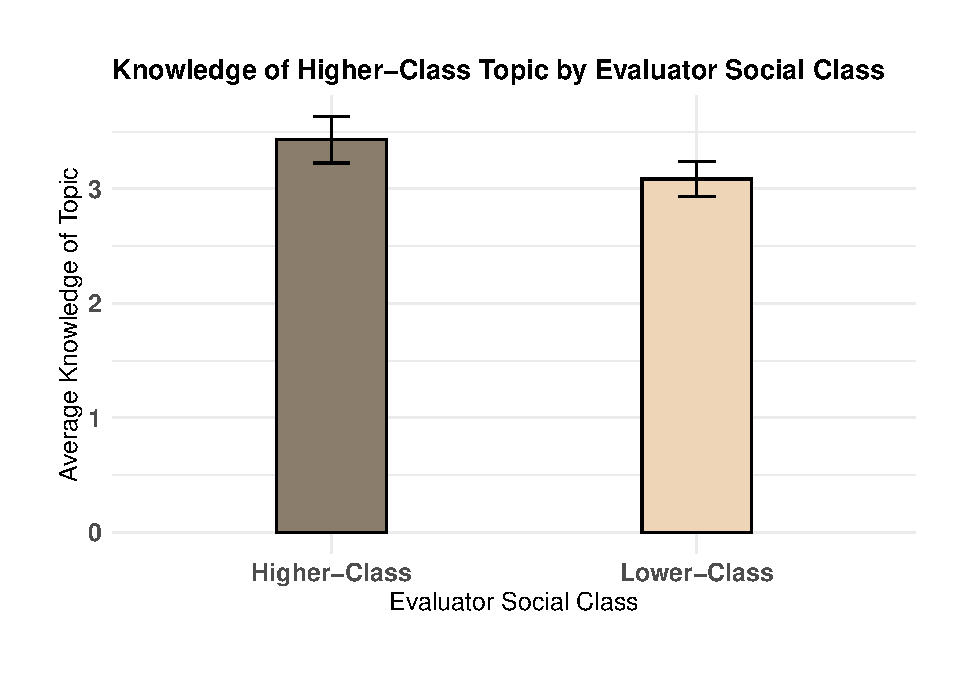
\includegraphics{sooyoun-pilot_files/figure-latex/bar-plot-high-1.pdf}
\caption{\label{fig:bar-plot-high}Knowledge of Higher-Class Topic by Evaluator Class}
\end{figure}

\begin{figure}
\centering
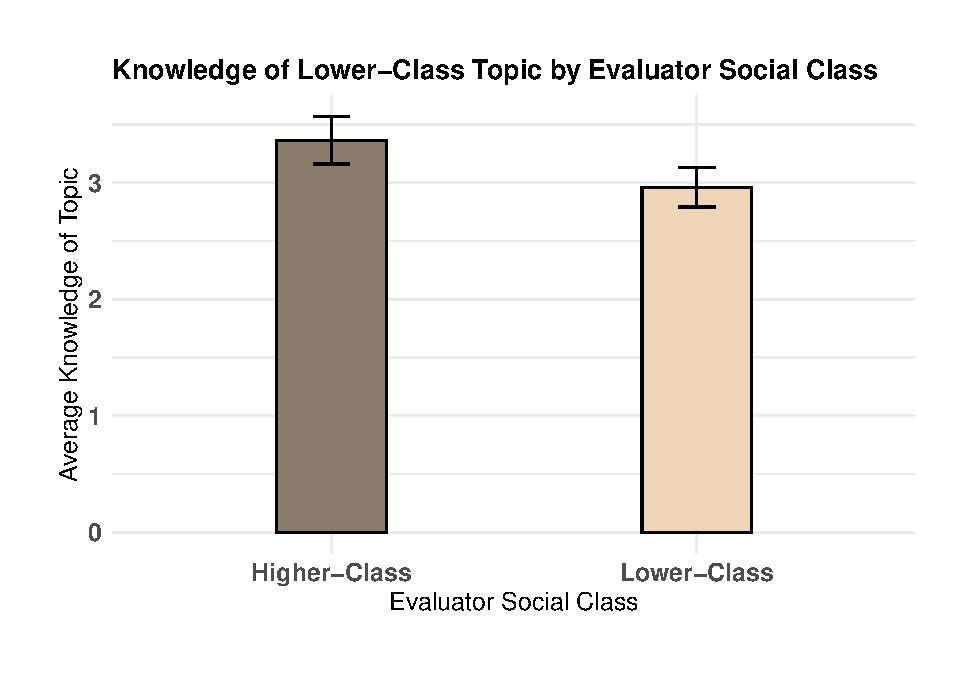
\includegraphics{sooyoun-pilot_files/figure-latex/bar-plot-low-1.pdf}
\caption{\label{fig:bar-plot-low}Knowledge of Lower-Class Topic by Evaluator Class}
\end{figure}

Further investigation through independent samples t-tests between higher-class and lower-class evaluators showed no significant difference in the knowledge regarding both conversation topics (Table~\ref{tab:t-test-evaluator}). Albeit the non-significant difference, bar plots for these analyses are presented (see Figure~\ref{fig:bar-plot-high}, Figure~\ref{fig:bar-plot-low}).

\hypertarget{listener-social-class-rating-comparison-by-vignette-type}{%
\subsection{Listener Social Class Rating: Comparison by Vignette Type}\label{listener-social-class-rating-comparison-by-vignette-type}}

\begin{table}[!h]
\centering
\caption{\label{tab:t-test-stat}Summary Statistics of Listener Social Class Rating by Vignette Type}
\centering
\begin{tabular}[t]{ccccc}
\toprule
Vignette & Mean & SD & sem & N\\
\midrule
Higher-Class & 6.57 & 1.91 & 0.35 & 30\\
Lower-Class & 4.83 & 1.72 & 0.29 & 36\\
\bottomrule
\end{tabular}
\end{table}

\begin{table}[!h]
\centering
\caption{\label{tab:t-test-listener}Difference in Listener Social Class Rating by Vignette Type}
\centering
\begin{tabular}[t]{lcccc}
\toprule
  & MeanDifference & t\_value & p\_value & df\\
\midrule
Higher- vs. Lower & 1.73333 & 3.84846 & 0.00029 & 59.06428\\
\bottomrule
\end{tabular}
\end{table}

Upon analyzing the dataset, I grouped observations by vignette type and calculated summary statistics for the listener's social class rating. The average inferred social class for the higher-class vignette was 6.57, with a standard deviation of 1.91 and a sample size of 30. Conversely, for the Lower-class vignette, the average was 4.83, with a standard deviation of 1.72 and a sample size of 36.

To further investigate the impact of vignette type on social class rating, a t-test was performed. The mean difference in perceived class ratings between higher- and lower-class vignettes was 2, with a t-value of 3.85 and a p-value of 0.00029. The findings were significant, indicating a strong effect of vignette type on perceived class. (see Table 6).

\begin{figure}
\centering
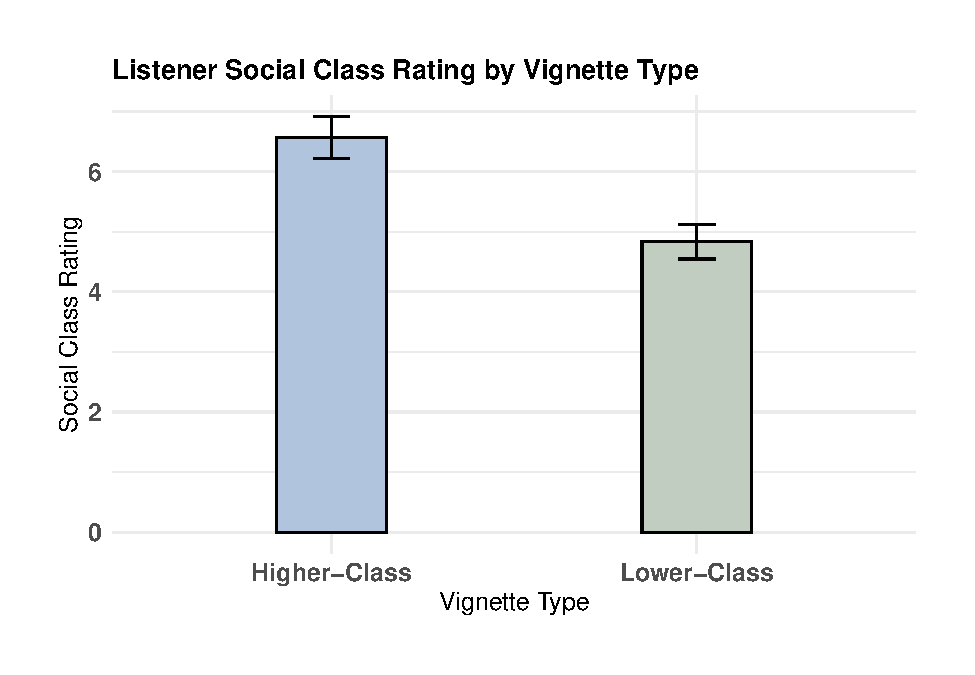
\includegraphics{sooyoun-pilot_files/figure-latex/bar-plot-listener-1.pdf}
\caption{\label{fig:bar-plot-listener}Listener Class Rating by Vignette Type}
\end{figure}

Figure~\ref{fig:bar-plot-listener} presents the average social class ratings of two vignettes and their associated standard errors. The average rating for the higher-class vignette type was 6.57 with a standard error of 0.35, whereas for the second vignette type, the average rating was 4.83 accompanied by a standard error of 0.29. The result underscores the significant difference (0.000294) in listener's social class ratings based on the topic of conversation.

\hypertarget{discussion}{%
\section{Discussion}\label{discussion}}

As Fiske and Markus (2012) note, social class profoundly impacts social identity, as it often dictates the social circles one interacts with and the societal norms one adheres to. The distinct life circumstances and standards build rigorous common ground within social class groups. Each norm, experience, and cultural reference builds unique knowledge bases (Lareau, 2014) and physical, psychological, and behavioral propensities (Kraus, Piff, Mendoza-Denton, Rheinschmidt, \& Keltner, 2012; Manstead, 2018; Piff, Kraus, \& Keltner, 2017).
Notably, in settings where diverse social identities interact, bridging these common grounds will be necessary for productive conversation. This would involve being aware of each other's social class background, predicting gaps in perspectives and knowledge, and explaining concepts as occasion demands (Allen, 2020). It is well known that speakers' language production reveals much about their awareness of the listener's knowledge. This study takes an additional step by illustrating how the very act of establishing new common ground also reveals the listener's social class. Considering that people from different social classes have access to different information, the listener design will enable inferences about social class.
By probing whether the speaker's words hint at the social class background of the listener, this study introduces one subtle and intricate way in which class information circulates during social interactions. This study also points out the broader societal consequences of status perception. Cuddy and colleagues (2008) showed that subtle social status cues can respectively predict impressions---for example, warmth and competence (i.e., Stereotype Content Model (SCM); (Durante, Tablante, \& Fiske, 2017)---which could influence interpersonal relationships and selection processes (Kraus, Park, \& Tan, 2017; Rivera \& Tilcsik, 2016; Stangor, 2016). In a large sense, unraveling the dynamics of social class signaling can yield meaningful insight into the barriers that may account for socioeconomic mobility.

\newpage

\hypertarget{references}{%
\section{References}\label{references}}

\begingroup
\setlength{\parindent}{-0.5in}
\setlength{\leftskip}{0.5in}

\hypertarget{refs}{}
\begin{CSLReferences}{1}{0}
\leavevmode\vadjust pre{\hypertarget{ref-allenTalkingSomeoneDifferent2020}{}}%
Allen, V. (2020). Talking with someone from a different social class requires more brain power, new research suggests. \emph{Daily Mail}.

\leavevmode\vadjust pre{\hypertarget{ref-bjornsdottirVisibilitySocialClass2017a}{}}%
Bjornsdottir, R. T., \& Rule, N. O. (2017). The visibility of social class from facial cues. \emph{Journal of Personality and Social Psychology}, \emph{113}(4), 530--546.

\leavevmode\vadjust pre{\hypertarget{ref-cuddyWarmthCompetenceUniversal2008}{}}%
Cuddy, A. J. C., Fiske, S. T., \& Glick, P. (2008). Warmth and competence as universal dimensions of social perception: {The} stereotype content model and the {BIAS} map. In \emph{Advances in experimental social psychology} (M. P. Zanna, Vol. 40, pp. 61--149). {Elsevier Academic Press}.

\leavevmode\vadjust pre{\hypertarget{ref-durantePoorWarmRich2017}{}}%
Durante, F., Tablante, C. B., \& Fiske, S. T. (2017). Poor but warm, rich but cold (and {Competent}): {Social} classes in the stereotype content model. \emph{Journal of Social Issues}, \emph{73}(1), 138--157.

\leavevmode\vadjust pre{\hypertarget{ref-fiskeFacingSocialClass2012}{}}%
Fiske, S. T., \& Markus, H. R. (2012). \emph{Facing social class how societal rank influences interaction}. {Russell Sage Foundation}.

\leavevmode\vadjust pre{\hypertarget{ref-krausSignsSocialClass2017}{}}%
Kraus, M. W., Park, J. W., \& Tan, J. J. (2017). Signs of social class: {The} experience of economic inequality in everyday life. \emph{Perspectives on Psychological Science}, \emph{12}(3), 422--435.

\leavevmode\vadjust pre{\hypertarget{ref-krausSocialClassSolipsism2012}{}}%
Kraus, M. W., Piff, P. K., Mendoza-Denton, R., Rheinschmidt, M. L., \& Keltner, D. (2012). Social class, solipsism, and contextualism: {How} the rich are different from the poor. \emph{Psychological Review}, \emph{119}(3), 546--572.

\leavevmode\vadjust pre{\hypertarget{ref-krausEvidenceReproductionSocial2019a}{}}%
Kraus, M. W., Torrez, B., Park, J. W., \& Ghayebi, F. (2019). Evidence for the reproduction of social class in brief speech. \emph{Proceedings of the National Academy of Sciences of the United States of America}, \emph{116}(46), 22998--23003.

\leavevmode\vadjust pre{\hypertarget{ref-lareauUnequalChildhoodsClass2014}{}}%
Lareau, A. (2014). \emph{Unequal childhoods: {Class}, race, and {Family Life}}. {University of California Press}.

\leavevmode\vadjust pre{\hypertarget{ref-mansteadPsychologySocialClass2018}{}}%
Manstead, A. S. (2018). The psychology of social class: {How} socioeconomic status impacts thought, feelings, and behaviour. \emph{British Journal of Social Psychology}, \emph{57}(2), 267--291.

\leavevmode\vadjust pre{\hypertarget{ref-piffUnpackingInequalityParadox2017}{}}%
Piff, P. K., Kraus, M. W., \& Keltner, D. (2017). Unpacking the inequality paradox: {The} psychological roots of inequality and social class. \emph{Advances in Experimental Social Psychology}, 53--124.

\leavevmode\vadjust pre{\hypertarget{ref-riveraClassAdvantageCommitment2016}{}}%
Rivera, L. A., \& Tilcsik, A. (2016). Class advantage, commitment penalty: {The} gendered effect of social class signals in an elite labor market. \emph{American Sociological Review}, \emph{81}(6), 1097--1131.

\leavevmode\vadjust pre{\hypertarget{ref-sebastianSpeechCuesSocial2018a}{}}%
Sebastian, R. J., \& Bouchard Ryan, E. (2018). Speech cues and social evaluation: {Markers} of ethnicity, social class, and age. \emph{Recent Advances in Language, Communication, and Social Psychology}, 112--143.

\leavevmode\vadjust pre{\hypertarget{ref-stangorStudyStereotypingPrejudice2016}{}}%
Stangor, C. (2016). The study of stereotyping, prejudice, and discrimination within social psychology: {A} quick history of theory and research. In \emph{Handbook of prejudice, stereotyping, and discrimination} (T. D. Nelson, pp. 3--27). {Psychology Press}.

\end{CSLReferences}

\endgroup


\end{document}
